\section{RQ1. Com que frequência \textit{breaking changes} surgem nos pacote clientes?}
\label{sec:rq1}

\subsection{Motivation}
\label{mot:rq1}

Atualmente, o \Gls{NPM} contém mais de 11 bilhões de downloads semanais e ultrapassa os 45 bilhões por mês. Os pacotes hospedados no \Gls{NPM} são usados por milhões de pessoas e projetos por todo o mundo. Eles são gratis, e fáceis de usar. Entretanto, uma simples \textit{release} que contenha um erro pode afetar uma quantidade imensa de pacotes. Isso se deve ao fato dos pacotes dependerem uns dos outros, direta ou indiretamente e, quando uma \textit{release} introduz \textit{breaking changes}, muitos pacotes podem ser afetados.

Para evitar estes erros, o \Gls{NPM} utiliza \textit{strings} de versionamento, baseadas no \Gls{SEMVER} para especificar as versões dos provedores. Isso permite que um provedor publique uma \textit{release} que contenha \textit{breaking changes}, mas que não afete os clientes das versões prévias. Entretanto, pesquisas mostram que a distinção entre \textit{breaking} e \textit{non-breaking changes} não é totalmente clara e pode ser difícil para o desenvolvedor decidir como incrementar a \textit{string} de versionamento a cada \textit{release} \cite{noregrets2018}. Assim sendo, entender com que frequência os pacotes provedores publicam \textit{releases} com \textit{breaking changes} pode ajudar os clientes a fazerem uma decisão melhor sobre como e quando atualizar a versão do provedor.

Para responder essa questão de pesquisa, serão analisados três pontos: 1) quantas vezes cada provedor publica uma \textit{release} que contém \textit{breaking changes} - e qual é a porcentagem de \textit{releases}; 2) em qual nível da \textit{string} de versionamento as \textit{breaking changes} são tipicamente introduzidas, de acordo com o \Gls{SEMVER} - \textit{major, minor} ou \textit{patch}; 3) qual o percentual de clientes que atualizam para uma versão com \textit{breaking changes}.

Para analisar todos esses pontos, os pacotes sorteados foram clonados do \textit{GitHub}, atualizado o \textit{index} e os arquivos na \textit{Working Tree} através do comando \textit{git checkout} com o \textit{timestamp} da \textit{release}, excluido o arquivo \textit{package-lock.json}, atualizado a versão de cada um dos provedores no \textit{package.json} e executado os comandos \textit{npm install} e \textit{npm test}. Todo esse processo foi executado automaticamente pela ferramenta \textit{BCDetect} \footnote{https://github.com/danielventurini/bcdetect}. Então, o resultado da execução -- sucesso ou erro -- foi salvo juntamente com as informações sobre a versão do \textit{Node.JS} que foi executado e que deveria ter sido executada, de acordo com o \textit{timestamp}. % essa parte das versões eu vou explicar melhor em um capítulo falando sobre a ferramenta.

\subsection{Approach}
\label{apr:rq1}
Um \textit{stack trace} contém as informações sobre as subrotinas de um programa. É comumente utilizado para certos tipos de \textit{debugs}, nos quais eles auxiliam a visualizar e rastrear um determinado evento/erro. Quando os comandos \textit{npm install} e \textit{npm test} resultam em erro, o \Gls{NPM} mostra o erro e todas as chamadas de função, incluindo as invocações para os provedores. A Figura \ref{fig:trace} mostra um exemplo genérico de um \textit{stack trace} mostrado pelo \Gls{NPM} após a ocorrência de um erro.

\begin{figure}
    \centering
    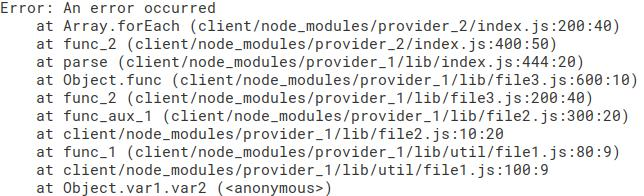
\includegraphics[scale=0.7]{figuras/stack_trace.jpeg}
    \caption{Generic stack-trace}
    \label{fig:trace}
\end{figure}{}

O \textit{stack trace} é a base para analisar um erro. A primeira etapa da análise de um erro é diferenciar entre um erro que foi causado pelo próprio pacote cliente, no qual não houve influência de nenhum provedor, portanto não caracteriza uma \textit{breaking change}, e um erro que foi causado por algum dos provedores, no qual se propagou para o pacote cliente e interrompeu-lhe a execução. Há duas maneiras que foi utilizada para realizar esta análise.

A primeira maneira foi verificar diretamente no \textit{stack trace} do erro e procurar as chamadas de função para os provedores. Quando não há chamada para os provedores no \textit{stack trace}, provavelmente o erro não se trata de uma \textit{breaking change}, porque nenhum provedor influenciou em nada na execução até acontecer o erro. Então, a falha pode estar apenas no código do cliente. Para confirmar isto, foi procurado no \textit{GitHub} do cliente os próximos \textit{commits} e verificado se o desenvolvedor realizou alguns \textit{commits} com a intenção de consertar algum erro - mensagens do tipo \textit{fix error}, \textit{fix bugs} etc. Se sim, o código do cliente foi alterado para verificar se as modificações presentes nos \textit{commits} realmente refletem a correção do erro. Então este caso foi confirmado como um \textit{non-breaking change} e foi descartado. Entretanto, alguns tipos de erros já indicam exatamente onde o erro aconteceu. São os \textit{SyntaxError} e \textit{ReferenceError}, no qual já se sabe onde e porque ocorreu. O Código \ref{cod:syntax:error} mostra um exemplo deste tipo de erro.

\begin{lstlisting}[style=Javascript, label=cod:syntax:error, caption={Código com um Reference Error}]
const a = 0 = 0;
\end{lstlisting}

Nesses casos, no qual o erro estava no pacote cliente, nem se fez necessário procurar por \textit{commits} no \textit{GitHub}. Apenas foi consertado diretamente no código do cliente e re-executado o comando que resultou em erro: \textit{install} ou \textit{test}. Isto para garantir que não houvesse um segundo erro que pudesse ser uma \textit{breaking change}.

A segunda maneira é quando o erro indicava a presença de \textit{breaking changes}. Isto se evidenciava quando havia chamadas para os provedores no \textit{stack trace}. Entretanto, as chamadas para \textit{frameworks} de teste, como o \textit{Mocha, Instanbul, Jasmine} entre outros, ou automatizadores de tarefas, o \textit{Grunt} por exemplo, não evidenciam diretamente a presença de \textit{breaking changes} uma vez que eles apenas iniciam a execução do pacote e deveriam estar ali. Porém, não foram totalmente descartados de apresentar \textit{breaking changes}. Assim, quando havia algum provedor no \textit{stack trace}, provavelmente se tratava de um caso de \textit{breaking change}.

O melhor local para se confirmar esta evidência é o \textit{GitHub}. Neste, os repositórios dos pacotes contêm todo o histórico de desenvolvimento. E muitas maneiras foram utilizadas para recuperar as informações necessárias. A primeira e mais fácil foi procurar nos arquivos registros de alterações, os comumente nomeados de \textit{CHANGELOG.md} ou \textit{HISTORY.md}. A proposta destes arquivos é manter uma lista ordenada cronologicamente das alterações significativas ao longo do desenvolvimento do projeto. E uma das informações muito importantes que são descritas nesses registos são as \textit{breaking changes}. Por exemplo, a versão \textit{5.0.0} do projeto \textit{Mocha} \footnote{https://github.com/mochajs/mocha} contém uma \textit{breaking change} que foi documentada no \textit{CHANGELOG.md}\footnote{https://github.com/mochajs/mocha/blob/master/CHANGELOG.md\#500--2018-01-17}. A Figura \ref{fig:bc_documentation} ilustra como foi realizada esta documentação.

\begin{figure}
    \centering
    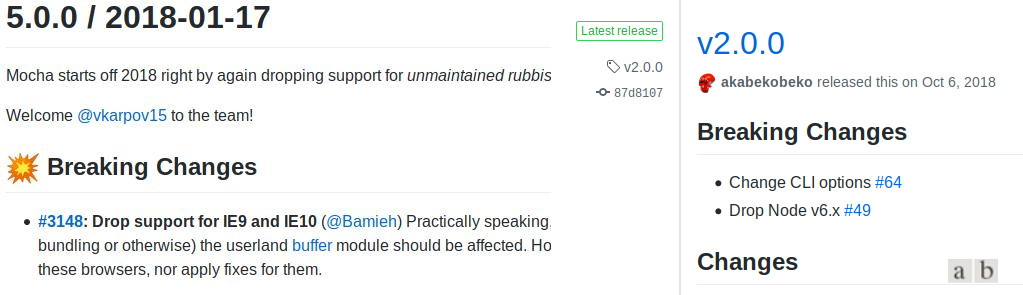
\includegraphics[scale=0.55]{figuras/bc_documentation.jpeg}
    \caption{Breaking Change documentation in README}
    \label{fig:bc_documentation}
\end{figure}{}

Assim, foi observado a versão do provedor que possivelmente causou o erro e foi verificado no seu \textit{CHANGELOG} -- caso existisse -- se contém alguma informação pertinente ao erro que foi apresentado pelo \gls{NPM} quando resultou em erro. Então foi salva as informações sobre este erro: a versão que iniciou, a versão que foi corrigido, uma breve descrição para facilitar a classificação da \textit{breaking change}, quem consertou o erro: cliente ou provedor; o tempo total até ser corrigido, quantas \textit{releases} o provedor levou para corrigir e em qual nível do \gls{SEMVER} o erro foi consertado.

Há ainda outros tipos de documentações parecidas com os \textit{changelogs}. Uma delas são as \textit{releases notes}. Elas são observações importantes sobre as alterações introduzidas por cada \textit{release}. Além disso, foi verificado nas \textit{issues} dos repositórios. Lá, muitas informações foram encontradas. E muito mais, pois há uma grande rede interligada de \textit{issues} e \textit{pull-requests} no qual uma \textit{issue} é marcada em outra \textit{issue}, que é marcada em um \textit{pull-request} e assim por diante. Deste modo, uma simples \textit{issue}/\textit{pull-request} contém muita informação.

Um ponto que foi muito importante para descobrir as versões que foram introduzidas as \textit{breaking changes} é a instalação de versões prévias e sucessivas dos provedores. Com isso, foi possível testar a partir de qual versão o erro foi introduzido e consertado e descobrir qual foi o verdadeiro provedor causador do erro. Também, alguns outros recursos foram utilizados para buscar as informações desta questão de pesquisa, tais como, o uso da ferramenta \textit{npm-diff}\footnote{https://github.com/danielventurini/npm-diff}, que provê os \textit{diff} do código entre duas \textit{releases} de um determinado projeto, no qual foi verificado o que realmente foi introduzido e o que foi removido com mais detalhes.

A Figura \ref{fig:step_analyze} exemplifica as técnicas utilizadas para responder esta questão de pesquisa.

\begin{figure}
    \centering
    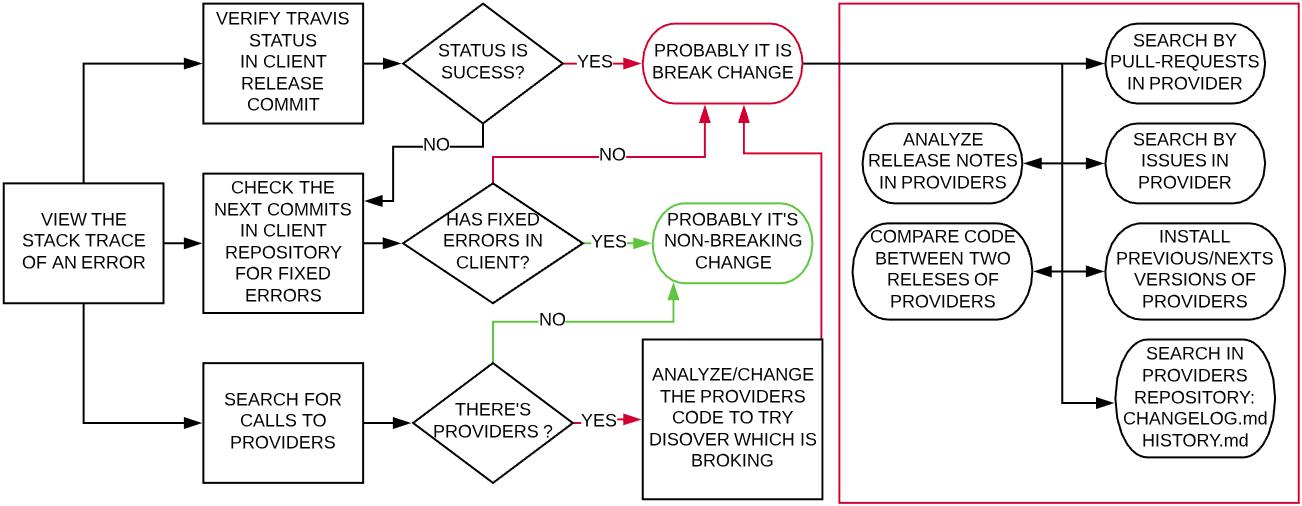
\includegraphics[scale=0.35]{figuras/step_analyze.jpeg}
    \caption{Passos para analisar um erro}
    \label{fig:step_analyze}
\end{figure}

Vale ressaltar que alguns sistemas integrados ao \textit{GitHub} auxiliaram na investigação. Esses sistemas são o \textit{Travis, Jenkins, Codeship, CicleCI} etc. que, quando o desenvolvedor realizou o \textit{commit}, esses sistemas executaram o \textit{npm install} e o \textit{npm test}. Isto colaborou da seguinte maneira: se o \textit{commit} da \textit{release} foi salvo o resultado do \textit{npm install} e \textit{npm test} como sucesso e, ao executá-los nesta pesquisa foi resultado em erro, indica que há uma \textit{breaking change}, uma vez que o código do cliente está no mesmo index do \textit{working tree}, apenas os provedores que foram atualizados e, para o range aceito, geraram erros, resultando em \textit{breaking changes}. Entretanto, nem todos os projetos utilizavam estes sistemas integrados, mas quando dispunham, foi de grande valia.

Outro detalhe importante se refere aos projetos que utilizavam algum tipo de sistemas terceiros como o \textit{MySql, CouchDB, Redis} etc. Então, quando foi gerado um erro pela falta de um destes, fez-se a habilitação destes e o pacote foi re-executado. Entretanto, quando os pacotes requeriam previamente uma configuração para executar, tais como a criação de tabelas em banco de dados, esta configuração foi feita, seguindo o modelo disponibilizado pelo desenvolvedor afim de realizar os teste, e novamente foi executado o pacote.

Então, para todas as \textit{releases} analisadas manualmente, foi salvo as seguintes informações:

\begin{enumerate}
    \item Em que local o erro foi documentado: \textit{issue, changelog, pull-request} etc;
    \item Quem consertou o erro: cliente ou providor;
    \item Em qual nível do \textit{SEMVER} o erro foi reparado;
    \item Quanto tempo o erro levou até ser corrigido; e
    \item Por quantas \textit{releases} o erro persistiu.
\end{enumerate}{}

\subsection{Findings}
\label{fin:rq1}

%---------------------------------------------------%
\section{RQ2. Quais são os problemas no pacote provedor que causam breaking change?}
\label{sec:rq2}

\subsection{Motivation}
\label{mot:rq2}

Uma vez que o provedor teve um comportamento inesperado pelo cliente, há \textit{breaking changes}. Isso pode causar uma mudança no comportamento do pacote cliente e, no pior caso, causar o encerramento de toda a execução se o cliente previamente na tratou um determinado erro. Entretanto, um cliente nunca espera que o provedor tenha um erro e, por isso, não fica tratando todas as chamadas para o cliente com \textit{try catch}. Assim, o cliente confia que o provedor esteja executando da maneira que foi especificado.

Um provedor pode conter múltiplos tipos de erros. Uma simples linha escrita semanticamente errada, por exemplo, pode causar no encerramento da execução, uma vez que os códigos \textit{Javascript} não são compilados. Entretanto, um erro pode não estar no provedor diretamente. Isto é devido ao fato deste contém um segundo provedor que seja o causador da \textit{breaking change}. Então, o erro é propagado do segundo provedor para o primeiro e, por fim, alcança o cliente. Isto é uma \textit{breaking change} transitiva e, na nossa pesquisa, é tratada como um caso normal de \textit{breaking change}.

Para responder essa questão de pesquisa, foi analisado caso a caso dos erros e as \textit{breaking changes} foram categorizadas pelo tipo da \textit{breaking change}. Também, os tipos foram quantificados pela categoria, pelo número de \textit{releases} afetadas e pelo número de clientes que sofreram com uma determinada categoria de \textit{breaking change}.

\subsection{Approach}
\label{apr:rq2}

Cada um dos casos de erro para os comandos \textit{npm install} e \textit{npm test} foram analisados manualmente. O objetivo era descobrir o real motivo que origino o erro e agrupa-los por suas similaridades. A Figura \ref{fig:error_category} mostra dois casos no qual uma função foi renomeada pelo provedor. Entretanto, previamente não está claro o real motivo dos erros, apesar da mensagem do \textit{stack trace}.

\begin{figure}[!h]
    \centering
    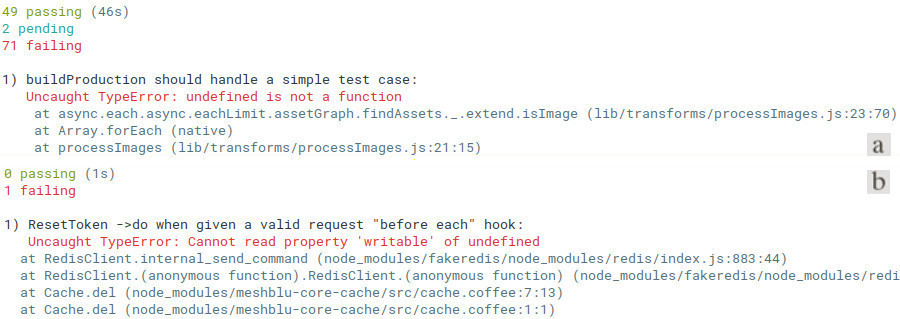
\includegraphics[scale=0.5]{figuras/error_category.jpeg}
    \caption{Two error caused by a renamed function}
    \label{fig:error_category}
\end{figure}

A mensagem do primeiro erro deixa claro que se trata de uma invocação a uma função inexistente, ou seja, o cliente tentou acessar uma variável como uma função quando esta não era. Mas, somente pela mensagem do \textit{stack trace} é possível deduzir que uma função foi renomeada no provedor. Já no segundo erro, o \textit{stack trace} não indica que o erro se trata de uma função renomeada. Somente após uma análise deste caso é que foi possível concluir que o erro aconteceu por uma função renomeada. Assim, apesar de mensagens de erro diferentes, foram classificados pelo seu real motivo para que fosse possível quantificar os principais problemas no código do provedor.

\subsection{Findings}
\label{fin:rq2}

%---------------------------------------------------%
\section{RQ3. Como os pacotes clientes se recuperam das breaking change?}
\label{sec:rq3}

\subsection{Motivation}
\label{mot:rq3}

Uma vez que uma \textit{breaking change} é introduzida o provedor deve se recuperar desta. Isso se faz necessário pois, no ecossistema \gls{NPM}, no qual centenas de milhares de pacotes estão conectados, uma simples \textit{release} com erro pode ocasionar na quebra de muitos clientes. Isto ocorreu com um pacote chamado \textit{left-pad}\footnote{https://blog.npmjs.org/post/141577284765/kik-left-pad-and-npm}. Este foi removido do \textit{NPM} por seu desenvolvedor e impactou milhares de projetos em apenas 2.5 horas incluindo \textit{babel}\footnote{https://github.com/babel/babel} e \textit{atom}\footnote{https://github.com/atom/atom}.

A responsabilidade para corrigir uma errônea \textit{release} é do provedor. Entretanto, as vezes, o provedor deixa dar a manutenção por algum motivo. Então, os clientes recebem esta responsabilidade, uma vez que o erro no seu provedor pode afetar os seus clientes. No caso do \textit{left-pad} o provedor nunca publicou uma nova \textit{release} e, para que todos os pacotes continuassem a executar normalmente, um dos clientes publicou um pacote com o mesmo nome e mesmo código, uma vez que a política para nomes de pacotes permitia este feito e o pacote original continha uma licença de código aberto.

Entretanto, nem sempre o cliente consegue resolver um problema no provedor. Isso se deve ao fato do cliente não ter conhecimento prévio do funcionamento interno do provedor ou por outros motivos. Assim, o cliente dificilmente irá conseguir ter sucesso quanto a resolução do erro no provedor. Então, uma alternativa para o cliente é alterar o seu provedor buscando por um que atenda as necessidades que não fora atendidas pelo provedor prévio.

Para responder a questão de pesquisa final, foi analisado três pontos: 1) o que aconteceu para que o provedor não pudesse consertar o erro; 2) como o cliente consertou o erro: no seu código ou notificando o provedor através de \textit{issues} e \textit{pull-requests}; 3) quantas vezes o cliente teve que realizar a correção dado que o provedor não a fez. Todas as informações sobre esta questão de pesquisa estão nos \textit{commits}, \textit{issues}, \textit{pull-requests}, \textit{changelogs} e \textit{releases-notes} dos repositórios do cliente e do provedor.

\subsection{Approach}
\label{apr:rq3}

Since the customer recovers from the error, there are two ways to know how it recoverer. The first way is when the provider fixes his code and the client just updates the string of versioning in \textit{package.json}, if it needs. To the provider fixes the error, one issue may be done in his repository. The second way is when the client must do some work to fix the code. In this case, the client can fix the provider code and do a pull-request or change his code to work with the provider. And of course, may have cases that anyone does nothing. There is a breaking change and it’s never been fixed.

Where information about this RQ is retrieved is \textit{GitHub}. This information can be found at \textit{CHANGELOG, release-notes, issues,} and \textit{pull-requests}. If the \textit{changelog} contains information about fixed errors, in general, the related \textit{issues} are marked. From these \textit{issues}, a lot of more information can be recovered, like \textit{pull-requests} that are also marked in the \textit{issue}, other \textit{issues}, commentaries and more. All of this information can help us to discover which one -- client or provider -- fixed the \textit{breaking change} and how it was fixed.

\textit{Commits} are the alternative to \textit{issues} when the search is in the client repository. The \textit{commits} contain all changes in files and the all updates providers in \textit{package.json}. Commits message like \textit{update dependencies, fix dependencies, fix errors} an so on, suggests that something about any dependencies was fixed. This information is very important, because, since the provider was fixed and the client just updates it, the commit messages can tell the reason for this update - or downgrade.

\subsection{Findings}
\label{fin:rq3}